%%%%%%%%%%%%%%%%%%%%%%%%%%%%%%%%%%%%%%%%%
% University Assignment Title Page 
% LaTeX Template
% Version 1.0 (27/12/12)
%
% This template has been downloaded from:
% http://www.LaTeXTemplates.com
%
% Original author:
% WikiBooks (http://en.wikibooks.org/wiki/LaTeX/Title_Creation)
%
% License:
% CC BY-NC-SA 3.0 (http://creativecommons.org/licenses/by-nc-sa/3.0/)
% 
% Instructions for using this template:
% This title page is capable of being compiled as is. This is not useful for 
% including it in another document. To do this, you have two options: 
%
% 1) Copy/paste everything between \begin{document} and \end{document} 
% starting at \begin{titlepage} and paste this into another LaTeX file where you 
% want your title page.
% OR
% 2) Remove everything outside the \begin{titlepage} and \end{titlepage} and 
% move this file to the same directory as the LaTeX file you wish to add it to. 
% Then add \input{./title_page_1.tex} to your LaTeX file where you want your
% title page.
%
%%%%%%%%%%%%%%%%%%%%%%%%%%%%%%%%%%%%%%%%%
%\title{Title page with logo}
%----------------------------------------------------------------------------------------
%	PACKAGES AND OTHER DOCUMENT CONFIGURATIONS
%----------------------------------------------------------------------------------------

\documentclass[12pt]{article}
\usepackage[english]{babel}
\usepackage[utf8x]{inputenc}
\usepackage{amsmath}
\usepackage{graphicx}
\usepackage[colorinlistoftodos]{todonotes}
\usepackage{hyperref}

\begin{document}

\begin{titlepage}

\newcommand{\HRule}{\rule{\linewidth}{0.5mm}} % Defines a new command for the horizontal lines, change thickness here

\center % Center everything on the page
 
%----------------------------------------------------------------------------------------
%	HEADING SECTIONS
%----------------------------------------------------------------------------------------

\textsc{\LARGE Università degli studi di Milano-Bicocca}\\[1cm] % Name of your university/college
\textsc{\Large Advanced Machine Learning }\\[0.3cm] % Major heading such as course name
\textsc{\large Final Project}\\[0.1cm] % Minor heading such as course title

%----------------------------------------------------------------------------------------
%	TITLE SECTION
%----------------------------------------------------------------------------------------

\HRule \\[0.4cm]
{ \huge \bfseries Floranet}\\[0.4cm] % Title of your document
\HRule \\[1.5cm]
 
%----------------------------------------------------------------------------------------
%	AUTHOR SECTION
%----------------------------------------------------------------------------------------

\large
\emph{Authors:}\\
Andrea Moleri - 902011 - a.moleri@campus.unimib.it \\   % Your name
Filippo Armani - 865939 - f.armani1@campus.unimib.it   \\[1cm] % Your name

% If you don't want a supervisor, uncomment the two lines below and remove the section above
%\Large \emph{Author:}\\
%John \textsc{Smith}\\[3cm] % Your name

%----------------------------------------------------------------------------------------
%	DATE SECTION
%----------------------------------------------------------------------------------------

{\large \today}\\[2cm] % Date, change the \today to a set date if you want to be precise

%----------------------------------------------------------------------------------------
%	LOGO SECTION
%----------------------------------------------------------------------------------------


\includegraphics{Images/logo}\\[1cm] % Include a department/university logo - this will require the graphicx package
 
%----------------------------------------------------------------------------------------

\vfill % Fill the rest of the page with whitespace

\end{titlepage}


%----------------------------------------------------------------------------------------
% ABSTRACT
%----------------------------------------------------------------------------------------

\begin{abstract}
This report presents Floranet, a deep learning-based approach aimed at developing models capable of correctly
identifying flower species from images while minimizing classification errors. The investigation focused on leveraging
transfer learning techniques with three base architectures: VGG16, DenseNet121, and InceptionV3. Various methodologies,
including full and partial freezing of network layers and the application of data augmentation were tested to evaluate
their impact on model performance. The result is a suite of models capable of solving the classification problem with
high test accuracy and low error propensity.

\end{abstract}

%----------------------------------------------------------------------------------------
% INTRODUCTION
%----------------------------------------------------------------------------------------

\section{Introduction}
The classification of images has become a cornerstone task in the field of machine learning and deep learning due to
its wide range of applications, from medical diagnostics to automated systems in agriculture. This project, titled
Floranet, focuses on the classification of flower species using the \href{https://www.robots.ox.ac.uk/~vgg/data/flowers/102/index.html}{Oxford Flower Dataset},
a dataset curated by Maria-Elena Nilsback and Andrew Zisserman. The dataset comprises 102 flower species, with the
number of images per species ranging from 40 to 258. These images present significant challenges due to variations in
scale, pose, lighting conditions, and intra-class diversity, as well as inter-class similarity.

\vspace{0.3cm}

The problem addressed by this project is the accurate classification of flower images into their respective species,
a task that requires robust models capable of handling the inherent complexity of the dataset. To tackle this problem,
transfer learning was used, a technique that leverages pre-trained deep learning models to improve the efficiency and
accuracy of new tasks. Specifically, three state-of-the-art architectures were utilized. The aim was to investigate the
strengths and limitations of each one, offering insights into the performance of different architectures when applied
to complex classification tasks. The subsequent sections will delve into the detailed methodology, experimental
results, and an analysis of the findings.

%----------------------------------------------------------------------------------------
% DATASETS
%----------------------------------------------------------------------------------------

\section{Datasets}
The dataset used in this project is the \href{https://www.robots.ox.ac.uk/~vgg/data/flowers/102/index.html}{Oxford Flower Dataset},
introduced in 2008 by Maria-Elena Nilsback and Andrew Zisserman. This dataset is designed for image classification tasks
and consists of 102 categories of flowers commonly found in the United Kingdom. The dataset includes three primary components:
image files (high-resolution flower images across all 102 categories), segmentation masks (masks that define flower regions
in the images), and labels (class labels for each image, provided in MATLAB format).

\vspace{0.3cm}

To prepare the dataset, the required files were downloaded, decompressed, and organized into meaningful directories.
A Python script was implemented to automatically handle this process, ensuring that any missing files were downloaded
and verified. Class labels were extracted from the MATLAB file (`imagelabels.mat`) and adjusted for Python’s zero-based
indexing. To facilitate analysis, a mapping between class indices and their corresponding flower names was created using
the official dataset documentation. The image files were matched to their labels and organized into a structured Pandas
DataFrame, where each row contains the image file name and the associated flower name. While this step is not strictly
necessary for training machine learning models, it aids in exploratory data analysis and ensures that the dataset is
correctly understood and annotated. The dataset's original benchmark, as described in its publication, utilized
hand-crafted features for classification. This project, however, leverages CNN-based approaches, exploring the
advantages of transfer learning with pre-trained deep learning architectures.

\vspace{0.3cm}

The dataset poses significant challenges due to its inherent imbalance: the most populated class contains 258 images
(Petunia), while the least populated class includes only 40 images (e.g., Pink Primrose). A quantitative analysis
[Fig.1] reveals that the average number of images per class is 80.28, with substantial variance indicating the presence
of class imbalance. To address this issue, a data augmentation strategy was implemented to ensure a more uniform distribution
across classes. The augmentation included transformations such as rotation, width shift, height shift, zoom, and flips.

\begin{figure}[h!]
    \centering
    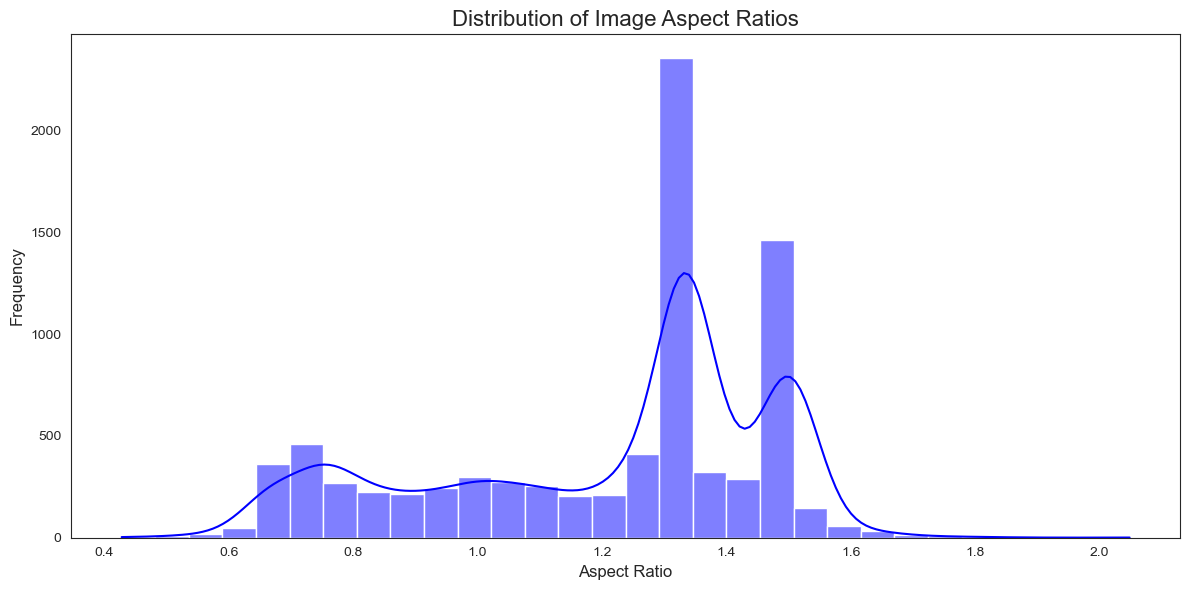
\includegraphics[width=\linewidth]{Images/Distribution of Image Aspect Ratios}
    \caption{Distribution of Image Aspect Ratios}
\end{figure}

Qualitative insights into the dataset were gained through visualizations. A bar plot [Fig.2] of class distributions highlights
the imbalance, while a subset of images from the top five most populated classes [Fig.3] showcases intra-class variability,
pose variations, and image quality. For instance, the Petunia class exhibits notable pose diversity, while inter-class
similarity is observed between Wallflower and Watercress. Additionally, intra-class variation is evident in the Water
Lily class, where samples within the same category differ significantly in appearance. Such variability may increase
the complexity of the classification task, necessitating robust feature extraction techniques.

\begin{figure}[h!]
    \centering
    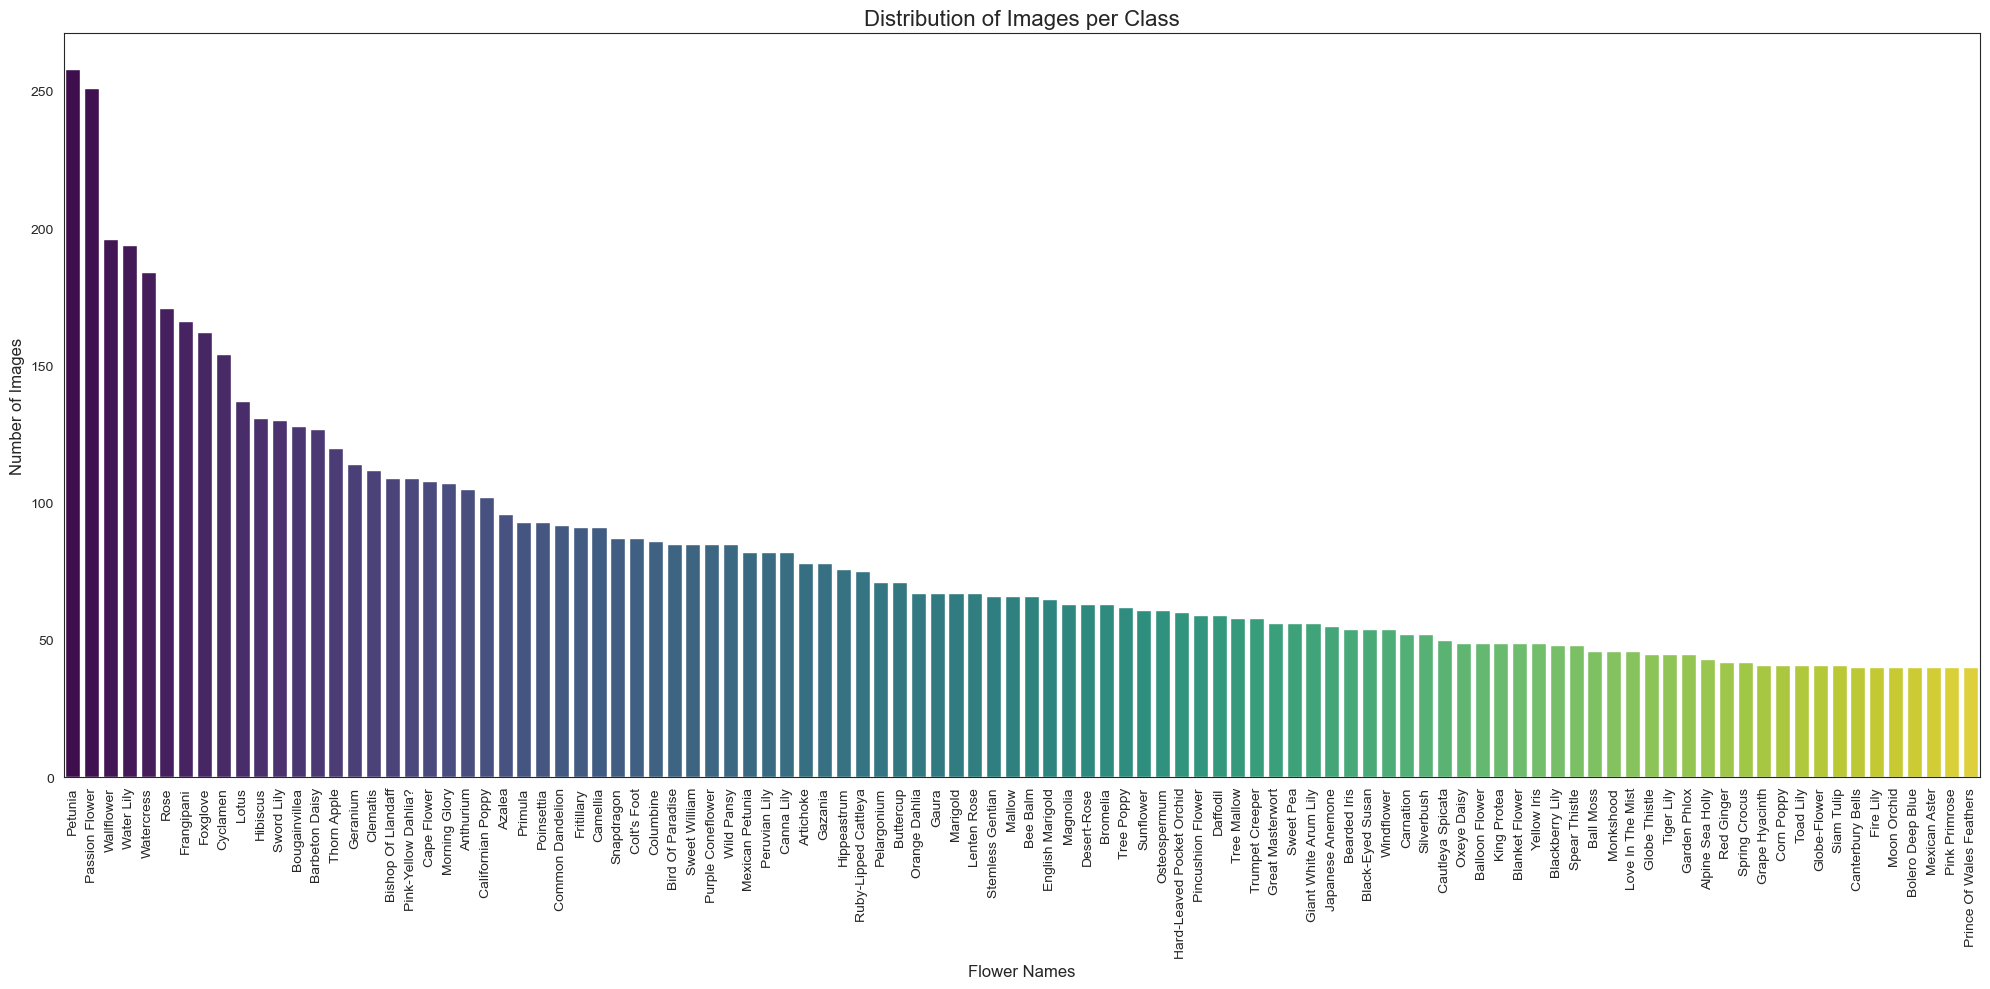
\includegraphics[width=\linewidth]{Images/Distribution of Images per Class}
    \caption{Distribution of Images per Class}
\end{figure}

\vspace{0.3cm}

To further understand the dataset's characteristics, the dimensions of all images were analyzed, yielding an average
resolution of approximately \(630 \times 534\) pixels. The aspect ratio distribution centers around 1.2, with minor
outliers. This uniformity in image dimensions simplifies preprocessing requirements but necessitates consistent
resizing for compatibility with convolutional neural networks. Furthermore, a comparison is made between flowers
extracted from 10 randomly selected classes, and flowers extracted from a specific class [Fig.4]. This visualization was made
to underscore the diversity within the dataset, and to highlight the consistency of samples for a particular category at the same time.

\begin{figure}[h!]
    \centering
    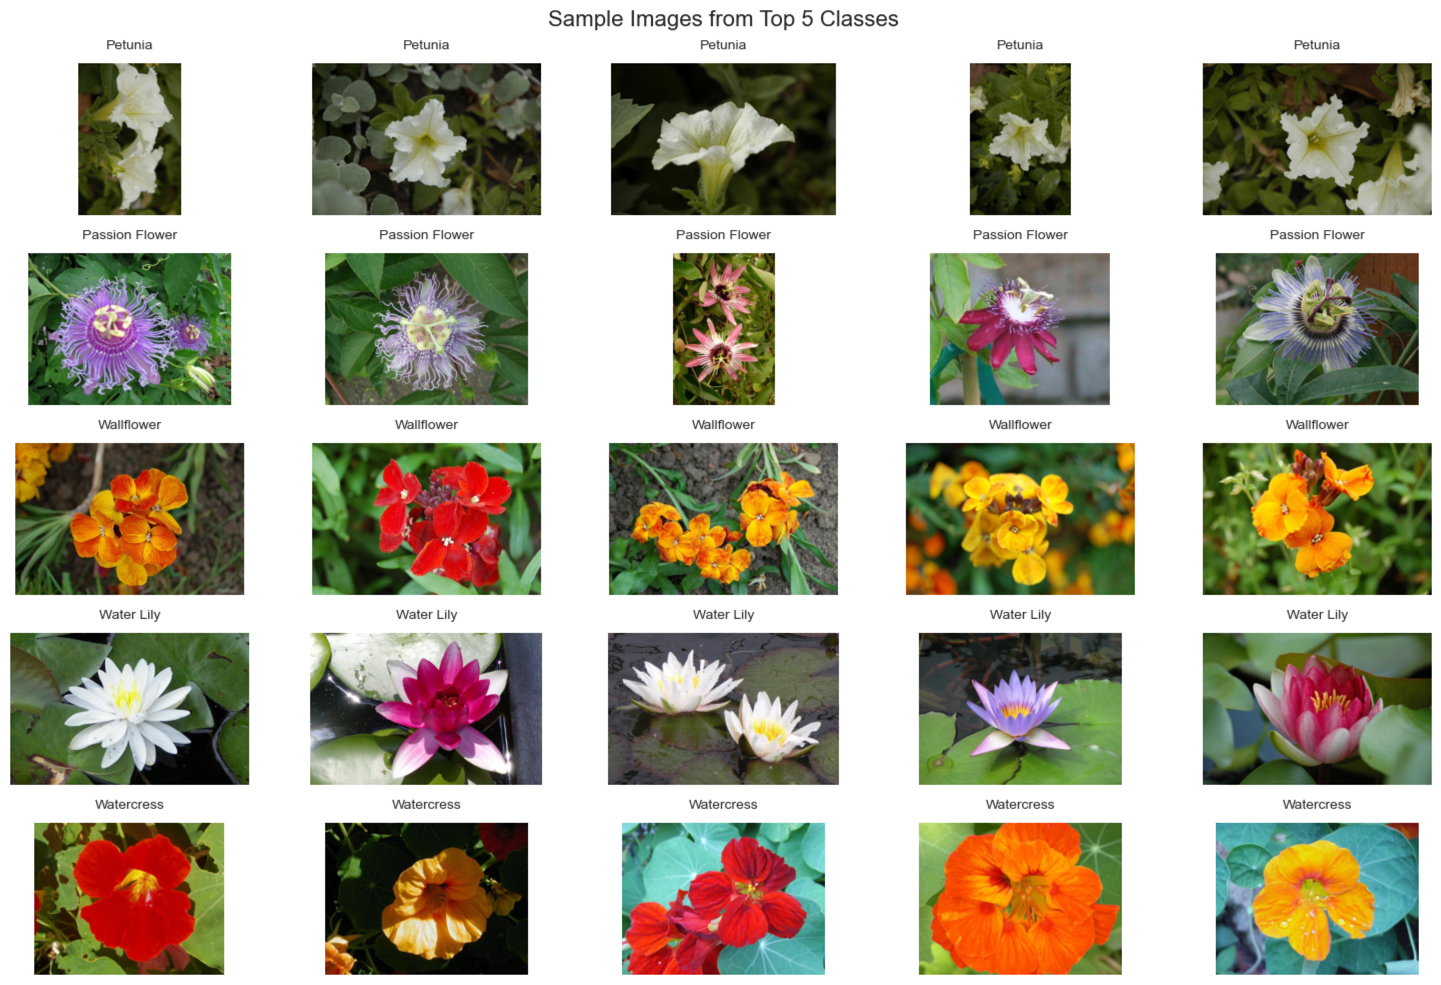
\includegraphics[width=\linewidth]{Images/Sample Images from Top 5 Classes}
    \caption{Sample Images from Top 5 Classes}
\end{figure}

\begin{figure}[h!]
    \centering
    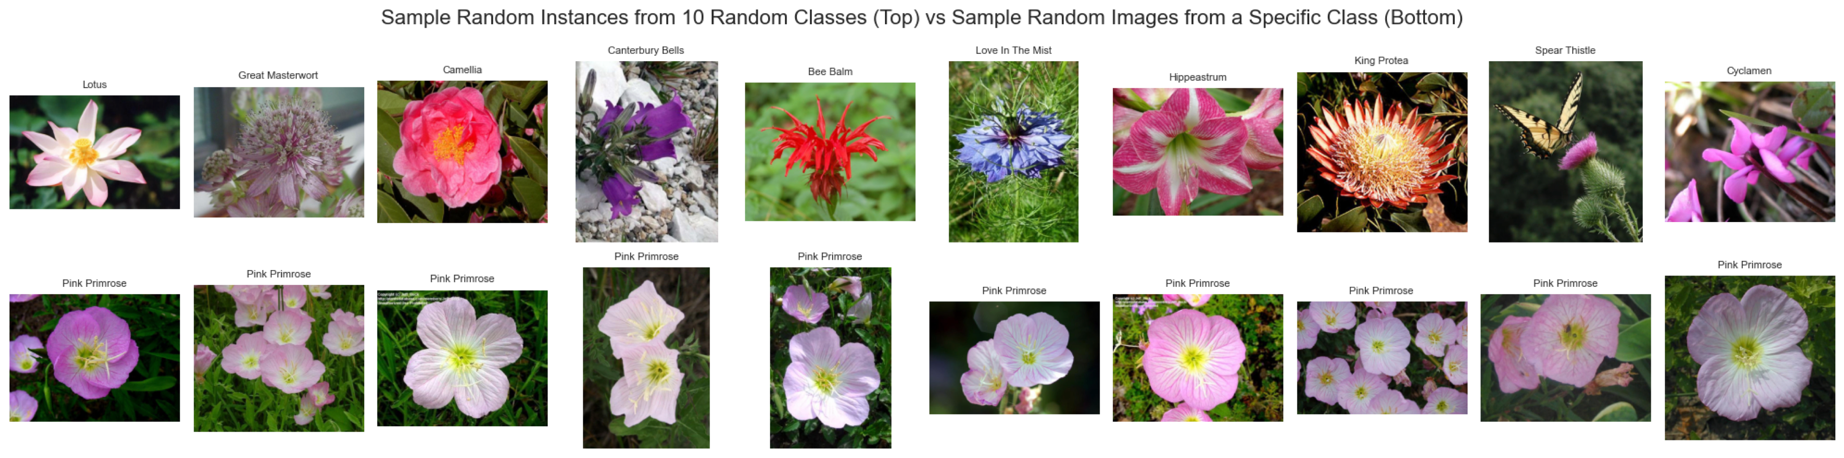
\includegraphics[width=\linewidth]{Images/Sample Random Instances from 10 Random Classes (Top) vs Sample Random Images from a Specific Class (Bottom)}
    \caption{Sample Images from Top 5 Classes}
\end{figure}

%----------------------------------------------------------------------------------------
% THE METHODOLOGICAL APPROACH
%----------------------------------------------------------------------------------------

\section{The Methodological Approach}

\subsection{Data Preprocessing}

The first step in the methodology involved preparing the dataset. The dataset was prepared by splitting it into
training, validation, and test sets (70\%, 15\%, and 15\%, respectively) using a stratified method to maintain class
balance. Despite some classes being over or underrepresented, this approach ensured proportional distribution across
subsets, minimizing biases and improving model generalization. One-Hot Encoding was applied to the target labels to
treat each class independently, and the preprocessed data was saved in CSV files for further processing.

\subsection{Model Architecture Selection}

For the classification task, three advanced convolutional neural network architectures were employed: VGG16,
DenseNet121, and InceptionV3. These models were selected due to their proven performance in image
classification tasks and their compatibility with transfer learning. Below, we elaborate on the key features and design
principles of each architecture, along with the motivations for their use in the context of the Oxford Flower Dataset.

\subsubsection*{VGG16}
VGG16, introduced by Simonyan and Zisserman, is characterized by its simplicity and depth. The architecture [Fig.5] employs a
sequence of small $3 \times 3$ convolutional filters, stacked in increasing depth, followed by max-pooling layers for
spatial dimensionality reduction. This design allows the model to capture complex hierarchical features while
maintaining manageable computational complexity. VGG16's consistent layer structure and relatively shallow gradient
paths make it a robust choice for transfer learning.

\begin{figure}[h!]
    \centering
    \includegraphics[width=\linewidth]{Images/VGG16}
    \caption{VGG16 Architecture}
\end{figure}

\subsubsection*{InceptionV3}
InceptionV3, a refined version of the Inception architecture introduced by researchers at Google, presents factorized
convolutions, batch normalization, and auxiliary classifiers to improve both training efficiency and accuracy.
The architecture [Fig.6] employs inception modules, which capture multiscale spatial features by performing convolutions of
varying kernel sizes in parallel. This multi-scale approach is ideal for the Oxford Flower Dataset, as flowers exhibit
diverse shapes and sizes. InceptionV3's ability to efficiently process such diversity while maintaining high
classification accuracy makes it a powerful choice for this task.

\begin{figure}[h!]
    \centering
    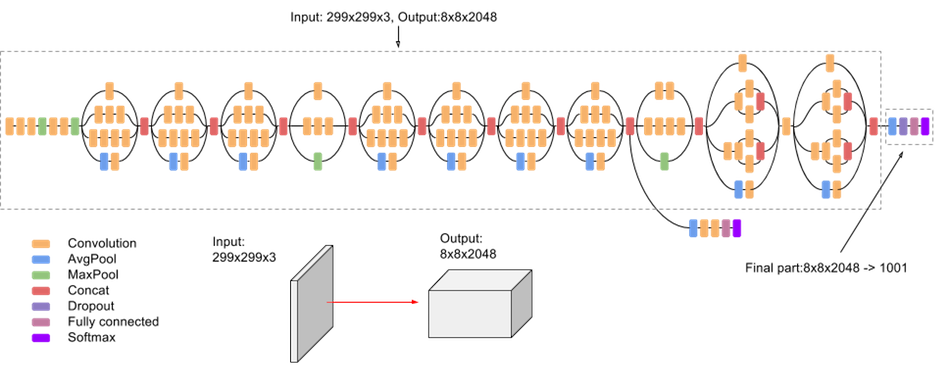
\includegraphics[width=\linewidth]{Images/InceptionV3}
    \caption{InceptionV3 Architecture}
\end{figure}

\subsubsection*{DenseNet121}
DenseNet121 leverages dense connectivity patterns where each layer is connected to every other layer within a block.
This connectivity encourages feature reuse, significantly reducing the number of parameters compared to traditional
architectures while improving gradient flow during training. The compactness and efficiency of the DenseNet121
architecture [Fig.7] make it particularly suitable for the classification task at hand, as the model can effectively learn
complex patterns in images, even in limited data scenarios.

\begin{figure}[h!]
    \centering
    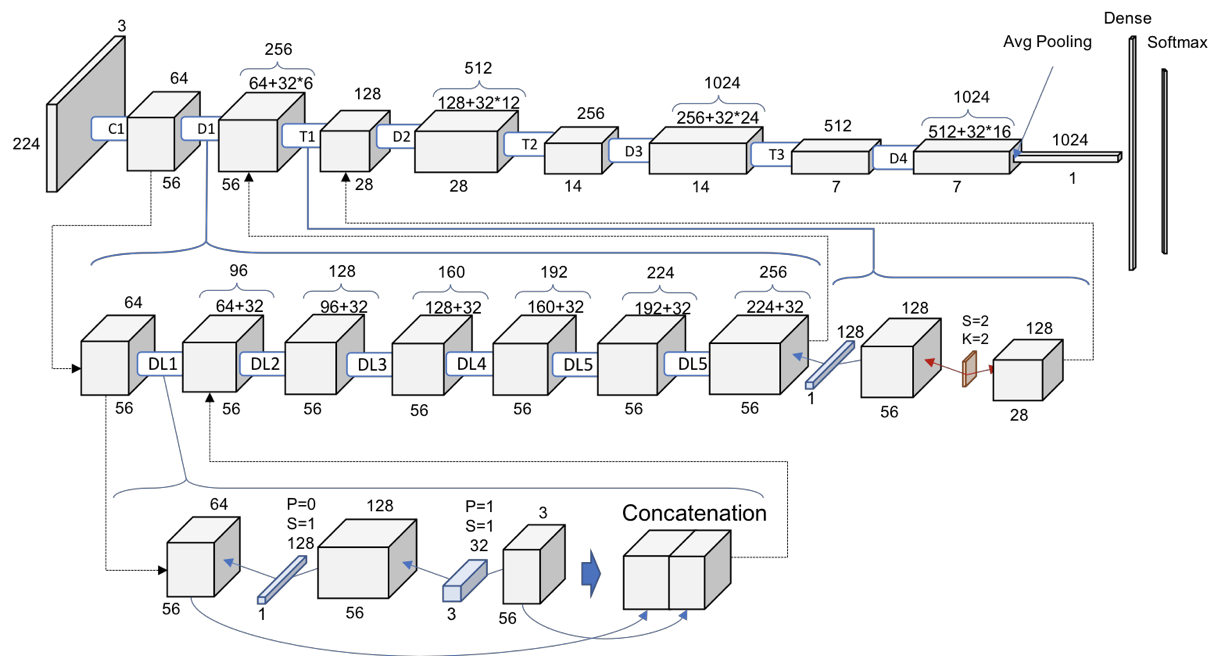
\includegraphics[width=\linewidth]{Images/Densenet121}
    \caption{DenseNet121 Architecture}
\end{figure}

\vspace{0.3cm}

\subsubsection*{Motivation for Model Selection}
The decision to use VGG16, DenseNet121, and InceptionV3 was guided by their complementary strengths. VGG16 provides a
solid baseline with its straightforward architecture, DenseNet121 offers parameter efficiency and feature reuse, and
InceptionV3 excels in capturing multiscale features i.e., the model can analyze details at different spatial scales and
handle the structural variety of flowers. Together, these models ensure a comprehensive approach to extracting the rich
visual information present in the Oxford Flower Dataset, leveraging transfer learning to address the dataset's relatively
small size effectively.

\subsection{Transfer Learning}

Transfer learning enables the use of pre-trained models that have already learned useful features from large, diverse
datasets such as ImageNet. In this project, each architecture was initialized with pre-trained weights and adapted for
the flower classification task. To prevent overfitting and improve generalization, several experiments were made for each network:

\begin{itemize}
    \item \textbf{Totally Frozen Base Model with Standard Training Data}: in this configuration, all layers are frozen, and the model is trained using the standard training data generator (`train\_generator`).
    \item \textbf{Totally Frozen Base Model with Augmented Training Data}: this configuration is similar to the first, but it uses data augmentation by employing the `train\_generator\_aug` data generator, which should help enhance generalization.
    \item \textbf{Partially Frozen Base Model with Standard Training Data}: in this case, `70\%` of the layers are frozen instead of `100\%`. The model is then trained with the standard training data generator.
    \item \textbf{Partially Frozen Base Model with Augmented Training Data}: this configuration mirrors the third, with `70\%` of the layers frozen, but it incorporates data augmentation during training
\end{itemize}

Furthermore, dropout layers were added after the dense layers to further mitigate overfitting and improve model
robustness. Each model was compiled using the Adam optimizer, with categorical cross-entropy as the loss function and
accuracy as the evaluation metric. The final classification was made using a softmax function.

%----------------------------------------------------------------------------------------
% RESULTS AND EVALUATION
%----------------------------------------------------------------------------------------

\section{Results and Evaluation}

After defining the experimental setups, it is possible to analyze the results using different diagnostic tools.
Among these we have two graphs [Fig.8] that show, on the left, the model metrics without validation curves, and on
the right, the model metrics with validation curves. We then have a table [Fig.9] that collects the salient values
of the experiments conducted, for example their duration, the values ​​of training accuracy, training loss,
validation accuracy, validation loss, test accuracy, test loss and the predictions made on the test set.

\begin{figure}[h!]
    \centering
    \includegraphics[width=\linewidth]{/Users/andreamoleri/PycharmProjects/Floranet/Images/combined_metrics.png}
    \caption{Training Metrics}
\end{figure}

\begin{figure}[h!]
    \centering
    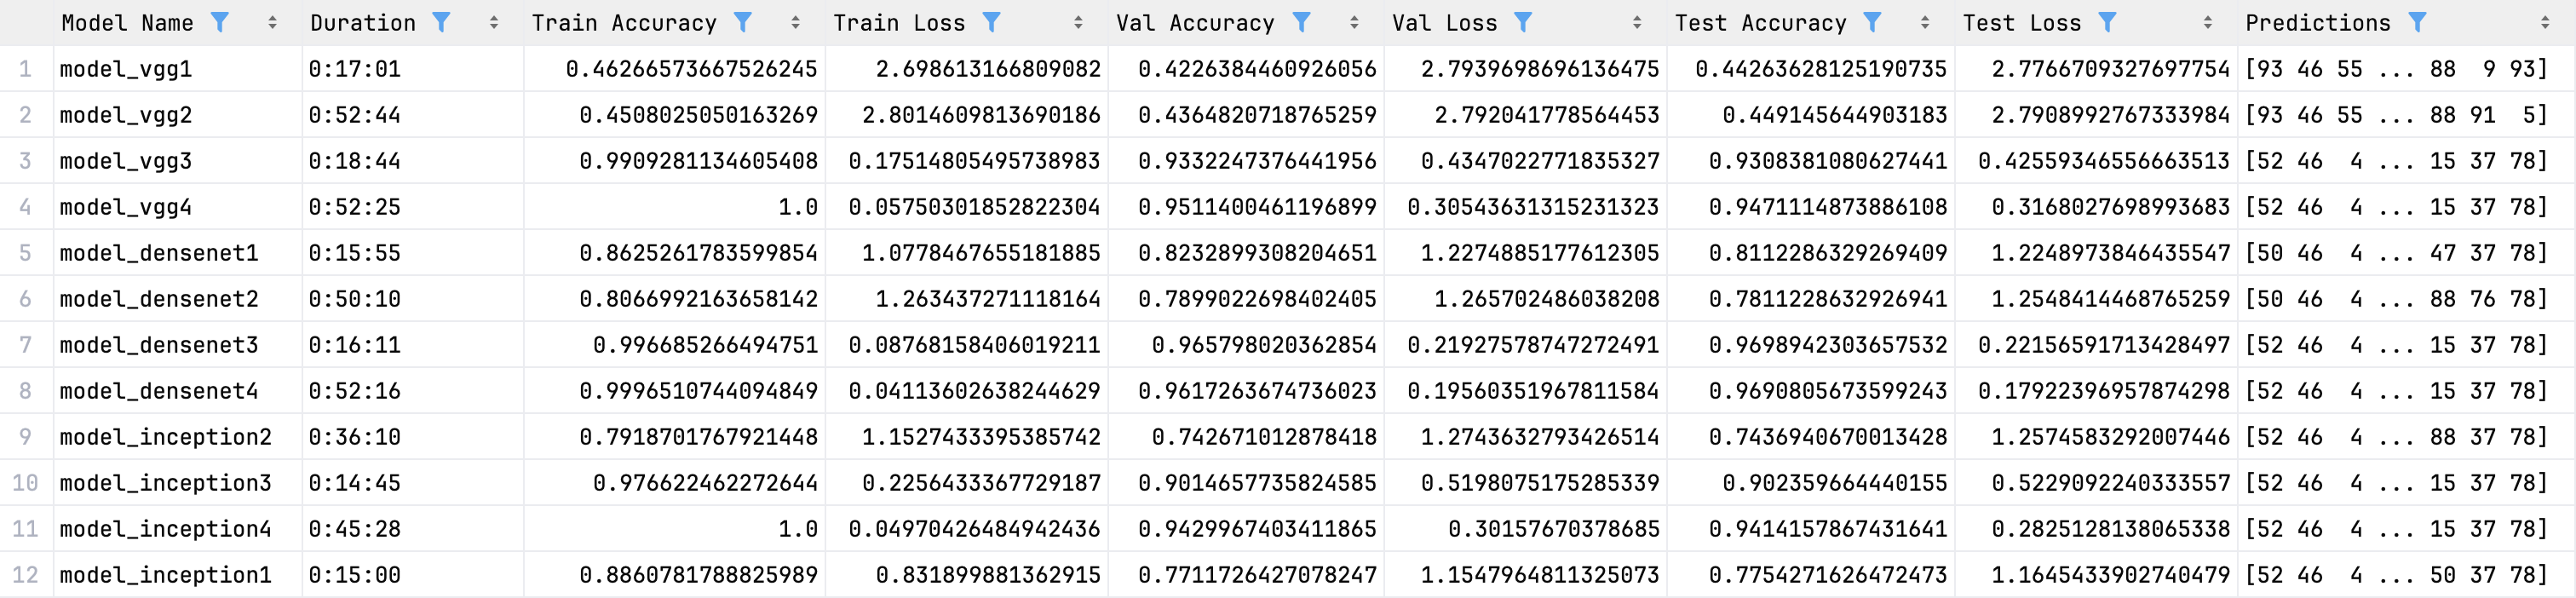
\includegraphics[width=\linewidth]{Images/Report}
    \caption{Experiments Report}
\end{figure}

\subsection{Evaluating the Training Metrics}

Evaluation of the training metrics revealed a consistent advantage for models with a `70\%` freeze over those with a
`100\%` freeze. These configurations demonstrated superior performance in terms of loss and accuracy, with data
augmentation showing only marginal influence. In the validation phase, models with a `100\%` freeze exhibited pronounced
underfitting, whereas `70\%` freeze configurations achieved better alignment between training and validation losses,
highlighting their stronger generalization capabilities.

\vspace{0.3cm}

InceptionV3 and VGG16 models followed similar trends, with `70\%` freeze configurations consistently outperforming
fully frozen counterparts. Data augmentation slightly improved training metrics but had limited impact overall.
Validation results for fully frozen models revealed more severe underfitting, only partially mitigated by data
augmentation, while `70\%` freeze models maintained superior validation accuracy.
DenseNet121 emerged as the most effective architecture, achieving the highest training accuracy and lowest loss,
especially with the `70\%` freeze configuration. This approach significantly improved metrics compared to fully frozen
models. The impact of data augmentation remained minor.

\subsection{Evaluating the Experiments Report}

The report that collects information on experiments shows additional information compared to the graphs. First of all,
let's recall that models ending in \("2"\) or \("4"\) use augmented data, while models ending in \("1"\) or \("3"\) employ non-augmented
data. Additionally, we remember that the "freeze\_percentage" value indicates the proportion of pre-trained layers
frozen during training, with models ending in \("3"\) and \("4"\) freezing 70\% of the layers, while models ending in \("1"\)
and \("2"\) freeze all pre-trained layers.

\vspace{0.3cm}

The experiments exhibit a high range of training accuracies, from as low as 45\% (model\_vgg2) to a perfect 99-100\%
(model\_vgg4, model\_densenet3, model\_densenet4, and so on). However, the high training accuracies observed must be
interpreted with caution, as they may indicate overfitting, particularly when paired with relatively lower validation/test
accuracies. In this regard, test accuracy is a key indicator of a model's ability to generalize to unseen data. We note
that the models with the higher freeze percentage show relatively lower test accuracies, indicating that these models
may not generalize well. Models that instead use a 70\% freeze percentage exhibit better generalization with test
accuracies nearing or above 90\%. In particular, model\_densenet3 demonstrate a remarkable test accuracy of 96.98\%.

\vspace{0.3cm}

The models with data augmentation tend to show slightly improved test performance compared to their non-augmented
counterparts. The augmentation process helps prevent overfitting by introducing variation in the data, which may
explain the superior test accuracies. This, however, comes at a cost: experiments without data augmentation take
around 15-20 minutes to train (using Google Colab's T4 GPU Hardware Accelerator), while experiments with data
augmentation take around 0 minutes to train.
From the analysis of the dataframe, we can also gather further insights. For example, loss values also provide insight
into model behavior. High training loss values paired with high test loss, such as in model\_vgg1, model\_vgg2, and
model\_inception1, suggest that these models struggle to fit the data properly. On the other hand, models like
model\_densenet3, model\_densenet4, model\_inception3, and model\_inception` exhibit lower loss values,
which align with their higher generalization abilities.

%----------------------------------------------------------------------------------------
% DISCUSSION
%----------------------------------------------------------------------------------------

\section{Discussion}

The conducted evaluations consistently demonstrate that the `70\%` freeze configuration outperforms other settings across all models.
In contrast, the `100\%` freeze configuration leads to underfitting, as the lack of flexibility inhibits the learning
of new features, resulting in suboptimal validation accuracy. These findings emphasize the importance of enabling
partial adaptability in the model layers for improved performance.

\vspace{0.3cm}

Data augmentation provided modest benefits, particularly for InceptionV3, where it reduced overfitting and enhanced
generalization. However, its overall impact on performance, notably in DenseNet121, was limited, indicating that robust
architectures might derive less benefit from such techniques for the task at hand. Given the increased training time
associated with augmentation, its application should be evaluated when the improvements in performance are marginal.
Models trained with data augmentation required significantly more time (up to 50 minutes) compared to those
without it (15-20 minutes).

\vspace{0.3cm}

DenseNet121 (with no data augmentation and 70\% freezing) emerges as the most effective architecture, achieving the
highest validation accuracy and a test accuracy of 96.98\%. The additional time needed for including data augmentation
in the training process (0:16:11 vs 0:52:16), in DenseNet, did not correspond to substantial accuracy gains, suggesting that augmentation's utility should
be weighed against its computational cost. To further confirm our hypotheses, a deeper analysis of model\_densenet3
will be conducted using its classification report and confusion matrix [Fig.10].

\begin{figure}[h!]
    \centering
    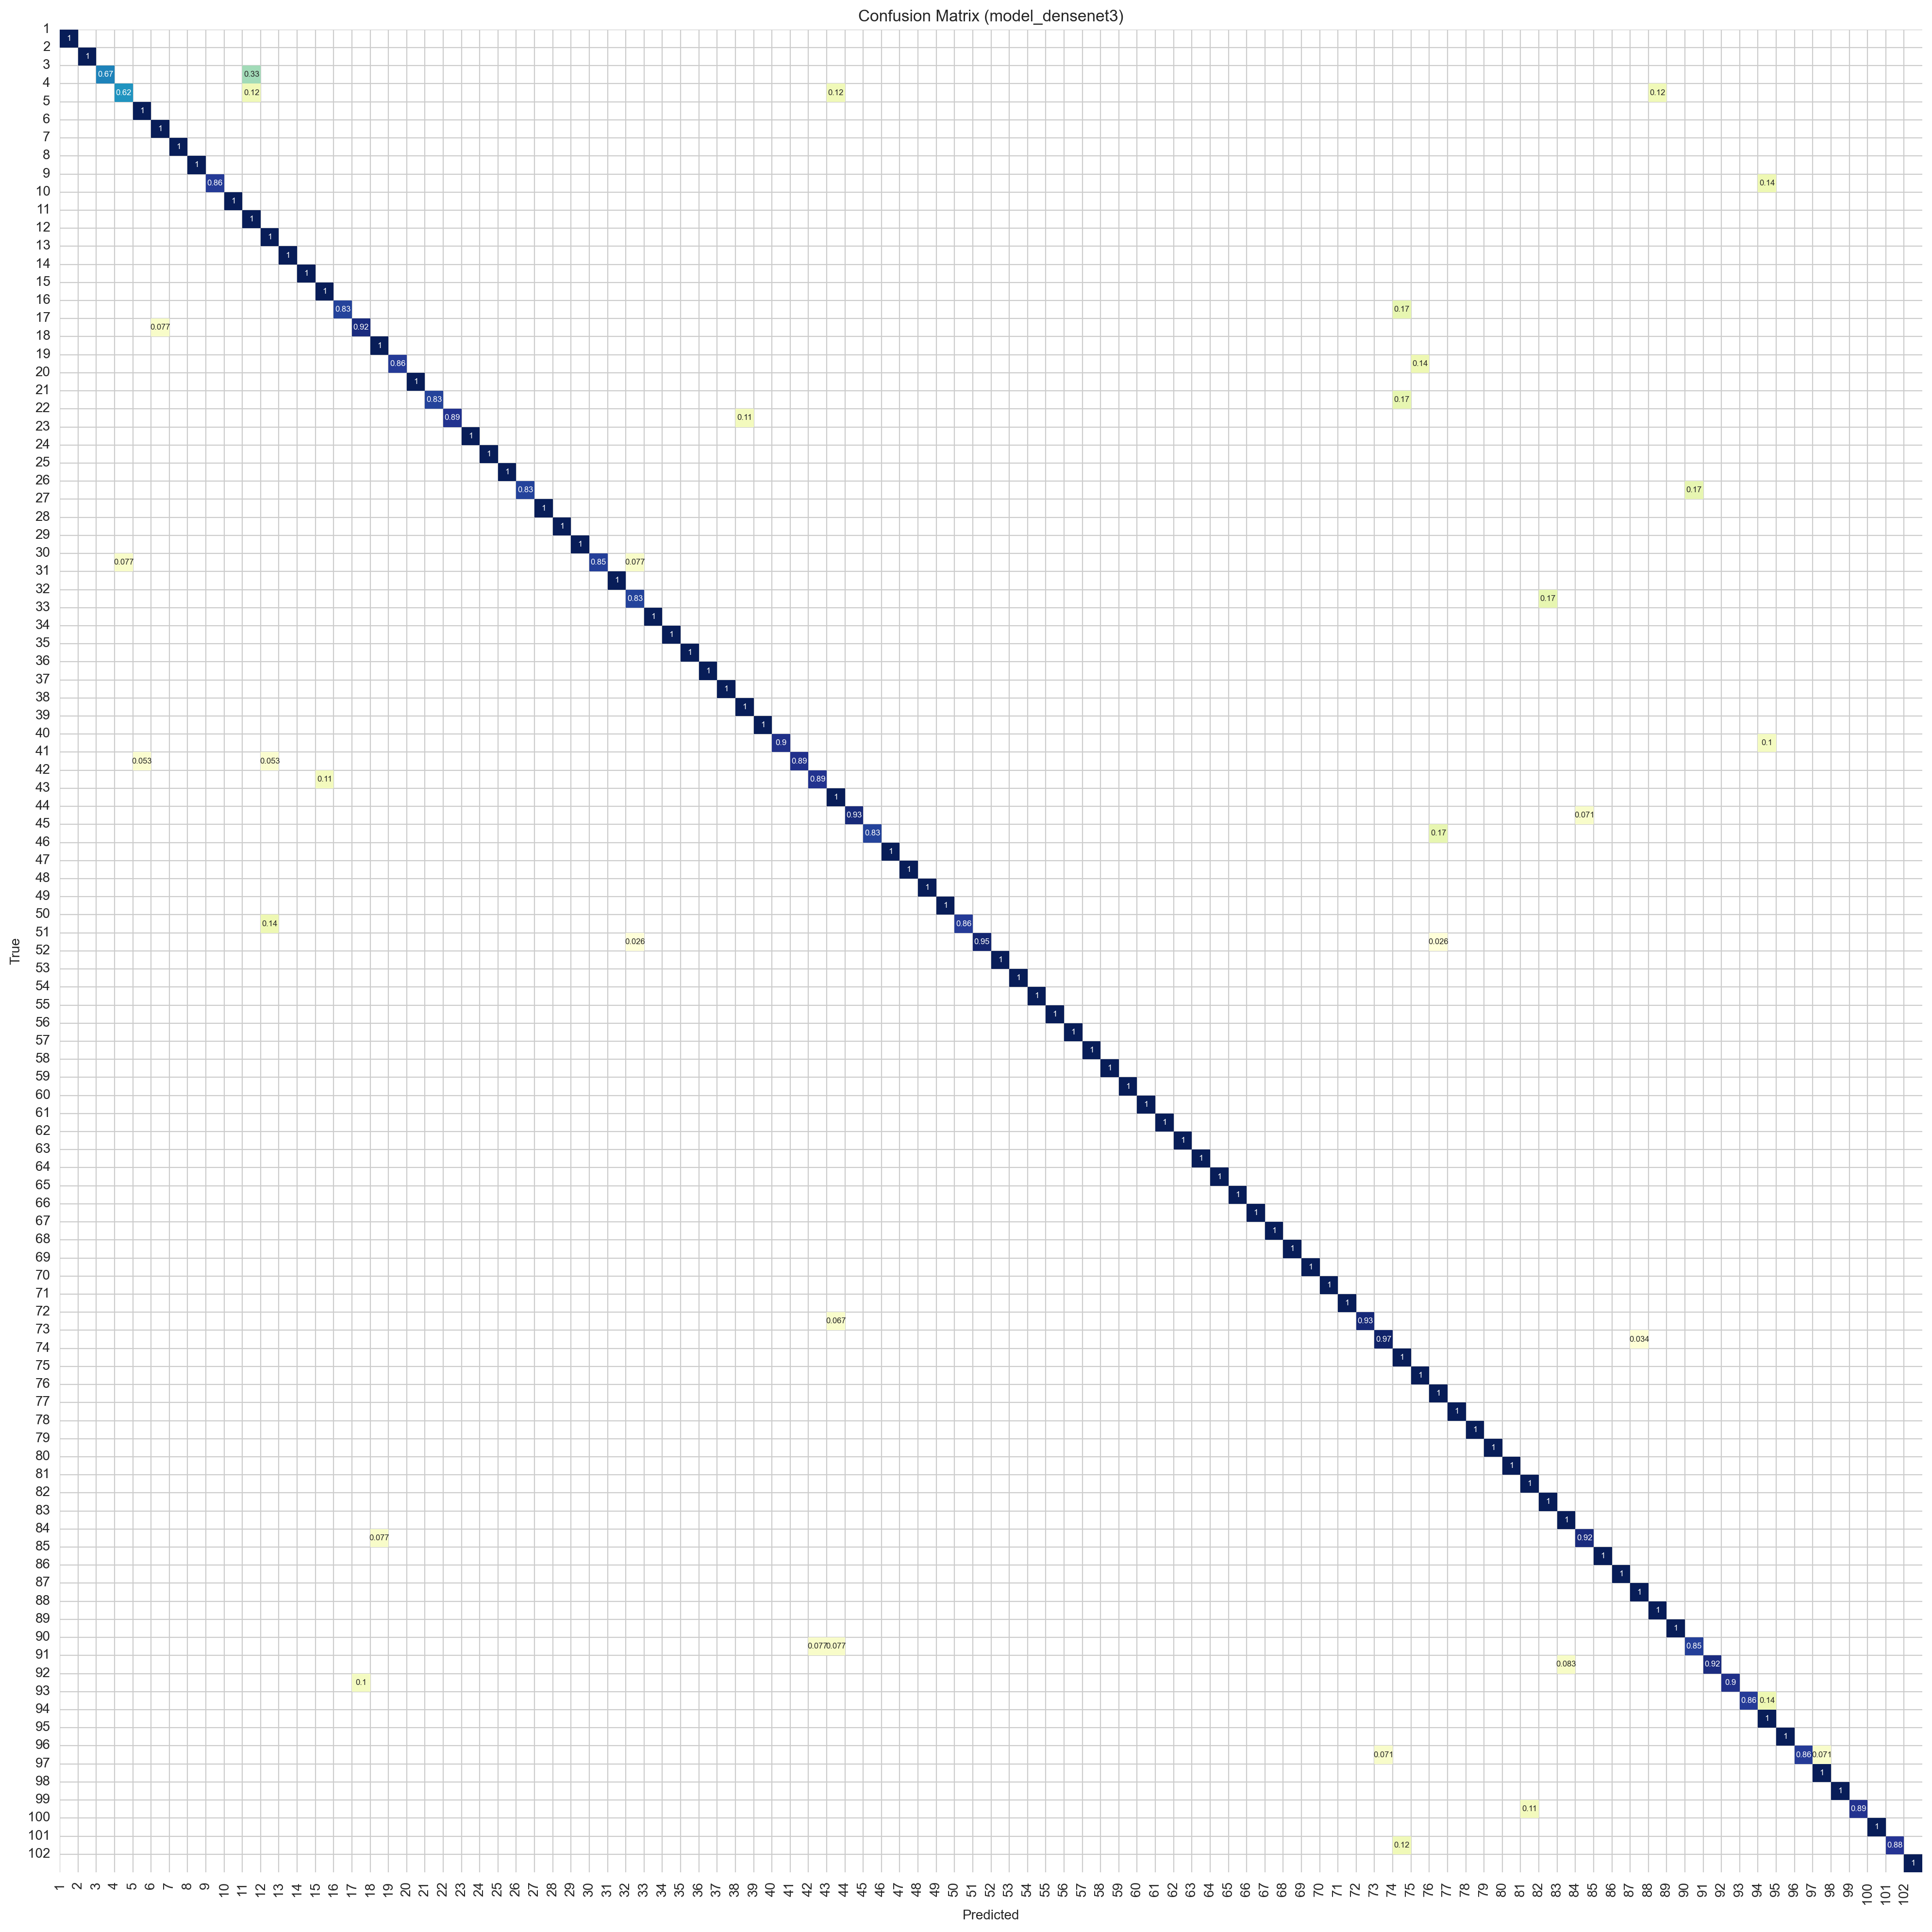
\includegraphics[width=\linewidth]{Images/Confusion Matrix}
    \caption{Confusion Matrix}
\end{figure}

The classification report for model\_densenet3 demonstrates outstanding performance across all categories, with
consistently high precision, recall, and F1-scores. Many classes achieve perfect scores (1.00), reflecting the model's
exceptional capability to accurately identify most samples. Both macro and weighted averages of 0.97 underscore its
balanced performance across all classes, avoiding significant bias. The model excels particularly with smaller classes,
where precision and recall are nearly flawless. Although minor variations exist, such as class 2 having a recall of 0.67
but maintaining an F1-score of 0.80, these do not detract from the model's overall robustness and versatility.
The confusion matrix further corroborates these findings, highlighting a dominant diagonal line indicative of high
accuracy across the majority of classes. Sparse off-diagonal elements and the light intensity of the few misclassifications
suggest errors are minimal and isolated rather than systematic. The absence of significant error clusters confirms that
the model has effectively learned discriminative features without displaying bias toward any particular category.

%----------------------------------------------------------------------------------------
% CONCLUSION
%----------------------------------------------------------------------------------------

\subsection{Conclusion}

This study evaluated the performance of three deep learning architectures across a range of experimental conditions.
The primary aim was to investigate the influence of various strategies and architectural choices on model performance,
generalization, and computational efficiency. Among the tested configurations, DenseNet121 with 70\% of its layers
frozen and no data augmentation was identified as the most effective model for the flower classification task. This
configuration achieved the highest validation and test accuracies, demonstrating an optimal balance between computational
efficiency and model performance. It offered robust results coupled with reduced training time, making it the most
efficient and effective solution for the given task, achieving a 96.98\% test accuracy.

%----------------------------------------------------------------------------------------
% REFERENCES
%----------------------------------------------------------------------------------------

\section*{References}

\begin{thebibliography}{99}

\bibitem{Nilsback2008} M.-E. Nilsback and A. Zisserman, ``Automated flower classification over a large number of classes,'' \textit{Proceedings of the Indian Conference on Computer Vision, Graphics and Image Processing}, pp. 722–729, 2008.

\bibitem{Russakovsky2015} O. Russakovsky, J. Deng, H. Su, J. Krause, S. Satheesh, S. Ma, and A. Berg, ``ImageNet large scale visual recognition challenge,'' \textit{International Journal of Computer Vision}, vol. 115, no. 3, pp. 211–252, 2015.

\bibitem{Pan2010} S. J. Pan and Q. Yang, ``A survey on transfer learning,'' \textit{IEEE Transactions on Knowledge and Data Engineering}, vol. 22, no. 10, pp. 1345–1359, 2010.

\bibitem{He2016} K. He, X. Zhang, S. Ren, and J. Sun, ``Deep residual learning for image recognition,'' in \textit{Proceedings of the IEEE Conference on Computer Vision and Pattern Recognition (CVPR)}, pp. 770–778, 2016.

\bibitem{Simonyan2014} K. Simonyan and A. Zisserman, ``Very deep convolutional networks for large-scale image recognition,'' in \textit{Proceedings of the International Conference on Learning Representations (ICLR)}, 2015.

\bibitem{Szegedy2015} C. Szegedy, W. Liu, Y. Jia, P. Sermanet, S. Reed, D. Anguelov, D. Erhan, V. Vanhoucke, and A. Rabinovich, ``Going deeper with convolutions,'' in \textit{Proceedings of the IEEE Conference on Computer Vision and Pattern Recognition (CVPR)}, pp. 1–9, 2015.

\bibitem{Zhang2017} L. Zhang, H. Zhang, and W. Li, ``A survey on data augmentation for deep learning-based image classification,'' \textit{IEEE Access}, vol. 5, pp. 7852–7863, 2017.

\bibitem{Shorten2019} C. Shorten and T. K. D. Khoshgoftaar, ``A survey on image data augmentation for deep learning,'' \textit{Journal of Big Data}, vol. 6, no. 1, pp. 60, 2019.

\bibitem{Krizhevsky2012} A. Krizhevsky, I. Sutskever, and G. E. Hinton, ``ImageNet classification with deep convolutional neural networks,'' in \textit{Proceedings of Advances in Neural Information Processing Systems (NeurIPS)}, pp. 1097–1105, 2012.

\bibitem{Chollet2017} F. Chollet, ``Xception: Deep learning with depthwise separable convolutions,'' in \textit{Proceedings of the IEEE Conference on Computer Vision and Pattern Recognition (CVPR)}, pp. 1251–1258, 2017.

\bibitem{Huang2017} G. Huang, Z. Liu, L. van der Maaten, and K. Q. Weinberger, ``Densely connected convolutional networks,'' in \textit{Proceedings of the IEEE Conference on Computer Vision and Pattern Recognition (CVPR)}, pp. 4700–4708, 2017.

\bibitem{Kingma2015} D. P. Kingma and J. Ba, ``Adam: A method for stochastic optimization,'' in \textit{Proceedings of the International Conference on Learning Representations (ICLR)}, 2015.

\bibitem{Li2019} X. Li, F. Zhu, S. Yang, and Y. Li, ``A comprehensive review on deep learning for image classification,'' \textit{Journal of Computational Biology}, vol. 26, no. 12, pp. 1161-1172, 2019.

\bibitem{Bengio2012} Y. Bengio, ``Learning deep architectures for AI,'' Foundations and Trends in Machine Learning, vol. 2, no. 1, pp. 1–127, 2012.

\bibitem{Goodfellow2016} I. Goodfellow, Y. Bengio, and A. Courville, \textit{Deep Learning}, MIT Press, 2016.

\end{thebibliography}


\end{document}




















